% =============================================================================
%  CRITIS 2026 -- FULL PAPER (<= 20 pp, Springer LNCS, in proceedings)
%  A Resilient Runtime-Verification Fabric for Security Monitoring of Critical
%  Edge-IoT Infrastructure. Reframed from the RV-Fabric (CloudNet) draft.
%
%  DOUBLE-BLIND: no author names/affiliations, NO acknowledgement, self-citations
%  neutralised to third person. Build: tectonic -X compile main.tex
%  All numbers are real (measured in ../paper_cloudnet/rv-fabric-impl/).
% =============================================================================
\documentclass[runningheads]{llncs}

\usepackage[T1]{fontenc}
\usepackage{amsmath,amssymb}
\usepackage{graphicx}
\usepackage{booktabs}
\usepackage{array}
\usepackage{colortbl}   % \rowcolor for shaded table section bands (xcolor already loaded via tikz)
\definecolor{rowtint}{gray}{0.93}
\newcolumntype{R}[1]{>{\raggedright\arraybackslash}p{#1}}
\usepackage{url}
\usepackage{xspace}
\usepackage{tikz}
\usetikzlibrary{arrows.meta,positioning,shapes,fit,backgrounds,calc}
\usepackage{pgfplots}
\pgfplotsset{compat=1.17}
\usepackage[hidelinks]{hyperref}
\usepackage{microtype}
\emergencystretch=5em   % absorb residual overfull lines (technical terms, inline math)
% --- reduce whitespace gaps from float placement ---
\raggedbottom
\renewcommand{\topfraction}{0.92}
\renewcommand{\bottomfraction}{0.85}
\renewcommand{\textfraction}{0.06}
\renewcommand{\floatpagefraction}{0.75}

\newcommand{\sys}{\textsc{RV-Fabric}\xspace}

\begin{document}

\title{A Resilient Runtime-Verification Fabric for Security Monitoring
       of Critical Edge-IoT Infrastructure}
\titlerunning{A Resilient RV Fabric for Critical Edge-IoT Security Monitoring}
\author{Anonymous Submission}
\authorrunning{Anonymous}
\institute{Anonymised for double-blind review}
\maketitle

\begin{abstract}
Protecting critical infrastructure increasingly depends on continuously verifying
large IoT fleets against formal security specifications at runtime. Yet the
runtime-verification (RV) pipelines proposed for this task are typically single-host
prototypes whose monitors read a shared log file, an architecture with no resilience
to the failures such deployments incur: a crash or overload silently drops events,
clock skew corrupts the ordering that metric temporal monitors require, a
time-triggered ``node has gone silent'' property cannot fire when the network itself
falls silent, and one slow consumer stalls the pipeline. Each failure is
\emph{silent}: the monitor keeps emitting verdicts over a corrupted view. We present
\sys, a resilient delivery layer that carries the hierarchy over two brokers (MQTT for
device ingest, a durable stream broker for backend delivery) and re-establishes five
continuity guarantees: durable delivery under post-persistence crashes, a trusted
event order, progress under total silence, consumer isolation, and flow control under
bounded overload, each holding as an invariant conditioned on broker durability. We
evaluate them under controlled fault injection (crashes, clock skew, network silence,
and overload) on a containerised testbed. Measured against a fault-free oracle using
the real MonPoly engine and tick-driven liveness detectors, the shared-log baseline
misses six of seven injected security incidents and reports each as an unqualified
all-clear, whereas \sys preserves all seven; two
openly published critical-infrastructure datasets (water-SCADA and IoT/IIoT) further
replay end-to-end through the real engine. Finally, \sys makes evidence completeness
part of the verdict: each verdict carries a status (sound, degraded, incomplete, or
unavailable) derived from delivery gaps, retention pressure, and liveness, so an
incomplete stream can no longer yield an unqualified all-clear.

\keywords{Critical infrastructure protection \and Resilience \and Runtime
verification \and IoT security \and Intrusion detection \and Situational
awareness \and Edge-cloud continuum}
\end{abstract}

% ============================================================================
\section{Introduction}
\label{sec:intro}
Security monitoring for the Internet of Things is moving off individual devices onto the
tiered edge-cloud continuum, where evidence from many devices must be collected, ordered,
and reasoned about beyond any single node~\cite{shi2016edge}. This matters because large
IoT fleets are now both critical infrastructure and a favoured attack surface:
internet-facing devices are routinely compromised and conscripted into coordinated
campaigns that a single device, seeing only its own traffic, cannot
detect~\cite{stellios2018iot,cavalli2024iotsec}. Runtime verification (RV), which
continuously checks a running system against explicit formal
specifications~\cite{rvsurvey,bartocci2018introduction}, suits such behaviour: unlike
signature- or learning-based intrusion detection, an RV monitor flags any execution that
violates a stated property and emits an auditable witness. Recent hierarchical designs
push this across a deployment's tiers, with lightweight per-device checks, per-gateway
aggregation, and fleet-wide temporal-logic correlation catching coordinated cross-device
attacks no single node can see~\cite{ares2026,csr2026}.

The verification logic of these designs is mature, but the delivery layer beneath
them is not, and for critical infrastructure that layer is where resilience is
won or lost. Published prototypes run on a single host, with every monitor reading
from one shared append-only log file. That arrangement suits a formal-methods
evaluation but collapses on the edge-cloud continuum:
\emph{(i)} device-to-gateway links are lossy, so records vanish before a monitor
ever sees them; \emph{(ii)} devices and gateways keep independent, skewing clocks,
breaking the monotone-timestamp assumption metric temporal-logic monitors
depend on; \emph{(iii)} time-triggered properties (``no device has reported for
$T$ seconds'') never fire when the network goes silent, because a log
with no new lines produces no events to advance the monitor's clock; and
\emph{(iv)} a single shared log serialises all consumers with no flow
control, so one slow monitor stalls the pipeline and the design does not scale
past a handful of devices. These failures are silent: the monitors keep emitting
verdicts from a corrupted view of the fleet, so a dropped or mis-ordered
security-relevant event may cause an attack to go unflagged, exactly the
continuity failure a critical-infrastructure operator cannot tolerate
(Fig.~\ref{fig:silent}).

\begin{figure}[t]
\centering
\footnotesize
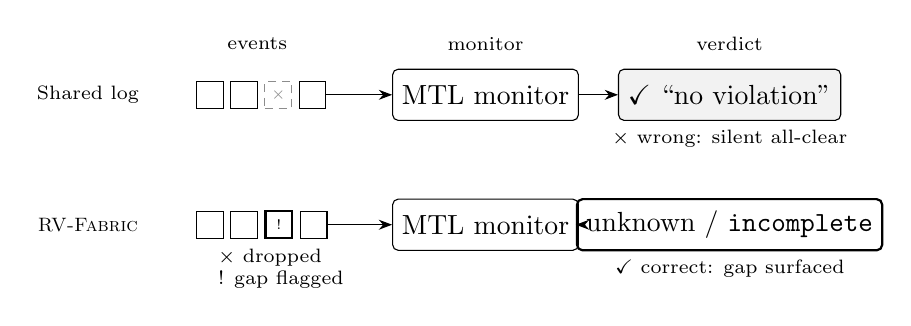
\begin{tikzpicture}[
  ev/.style={draw, minimum size=3.4mm, inner sep=0pt},
  drop/.style={ev, draw=black!45, densely dashed, text=black!45},
  gap/.style={ev, thick},
  mon/.style={draw, rounded corners=2pt, minimum height=6.5mm, minimum width=15mm, align=center},
  vbad/.style={draw, rounded corners=2pt, minimum height=6.5mm, minimum width=26mm, align=center, fill=black!5},
  vok/.style={draw, rounded corners=2pt, minimum height=6.5mm, minimum width=26mm, align=center, thick},
  lbl/.style={font=\scriptsize, align=left, text=black},
  a/.style={-Stealth}]
% fixed grid columns: events / monitor / verdict
\def\mx{3.5}\def\vx{6.6}\def\ry{0.4}\def\fy{-1.25}\def\toff{0.56}
% column headers
\node[lbl] at (0.6,1.05) {events}; \node[lbl] at (\mx,1.05) {monitor};
\node[lbl] at (\vx,1.05) {verdict};
% Row 1: shared log -> silent failure
\node[lbl] (t1) at (-1.55,\ry) {Shared log};
\node[ev] (x1) at (0,\ry) {}; \node[ev,right=0.8mm of x1](x2){};
\node[drop,right=0.8mm of x2](x3){\tiny$\times$}; \node[ev,right=0.8mm of x3](x4){};
\node[mon] (m1) at (\mx,\ry) {MTL monitor};
\node[vbad] (v1) at (\vx,\ry) {\checkmark\ ``no violation''};
\draw[a](x4)--(m1); \draw[a](m1)--(v1);
\node[lbl,align=center] at (\vx,\ry-\toff) {$\times$ wrong: silent all-clear};
% Row 2: fabric -> surfaced
\node[lbl] (t2) at (-1.55,\fy) {\sys};
\node[ev] (y1) at (0,\fy) {}; \node[ev,right=0.8mm of y1](y2){};
\node[gap,right=0.8mm of y2](y3){\tiny!}; \node[ev,right=0.8mm of y3](y4){};
\node[mon] (m2) at (\mx,\fy) {MTL monitor};
\node[vok] (v2) at (\vx,\fy) {unknown / \texttt{incomplete}};
\draw[a](y4)--(m2); \draw[a](m2)--(v2);
\node[lbl,align=center] at (\vx,\fy-\toff) {\checkmark\ correct: gap surfaced};
% glyph key, under the events column
\node[lbl,align=left] at (0.9,\fy-\toff) {$\times$ dropped\\{!} gap flagged};
\end{tikzpicture}
\caption{The failure mode \sys removes. On a shared log a dropped or mis-ordered event
is invisible to the monitor, which keeps emitting ``no violation'' over a corrupted view
(a \emph{silent} failure); \sys surfaces the breach through event-id gaps, downgrading
the verdict to $(\mathsf{unknown},\mathsf{incomplete})$ (Sect.~\ref{sec:guarantees}).}
\label{fig:silent}
\end{figure}

\paragraph{Contributions.} This paper makes four contributions.
\begin{itemize}
\item \sys, a resilient delivery layer that carries an unchanged three-layer monitoring
      hierarchy~\cite{ares2026,csr2026} across the edge-cloud continuum, re-establishing
      the delivery, ordering, liveness, isolation, and flow-control guarantees a shared
      log cannot provide (Sect.~\ref{sec:arch}).
\item A threat model for verification-grade monitoring that maps a tiered
      network/device/gateway adversary to its mitigation, with the five continuity
      properties stated as broker-contingent invariants, each closing a documented
      shared-log failure (Sects.~\ref{sec:threatmodel}--\ref{sec:guarantees}).
\item An evidence-aware verdict model, with a conditional-soundness proposition, that
      attaches a completeness status to every verdict so a degraded stream can no longer
      produce an unqualified all-clear (Sect.~\ref{sec:guarantees}).
\item An evaluation quantifying the restored properties under crash, clock skew, silence,
      and overload, including verdict preservation against a fault-free oracle, and
      replaying two critical-infrastructure datasets through the real MonPoly engine
      (Sects.~\ref{sec:eval},~\ref{sec:casestudy}).
\end{itemize}

\paragraph{Novelty.} \sys makes the \emph{completeness of the evidence stream} an
explicit part of runtime-verification semantics: each verdict carries a continuity
status derived from delivery, ordering, retention, and liveness evidence
(Sect.~\ref{sec:guarantees}), so a corrupted or incomplete stream can no longer produce
an unqualified all-clear, coupling transport resilience to verdict trustworthiness.

% ============================================================================
\section{Background and the \sys Architecture}
\label{sec:background}\label{sec:arch}
This section introduces the hierarchical monitoring workload \sys carries and the
single-host shared-log prototype it replaces, then derives from each layer's
assumptions the transport requirements the fabric must meet.

\paragraph{The three-layer hierarchy.}
\sys distributes a hierarchical monitoring workload across three tiers, each seeing a
wider slice of the fleet than the one below. \emph{Layer~1 (L1)}, on or beside each
device, runs stateless per-event sanity checks (payload size, publish rate, timestamp
monotonicity) and emits a compact per-window verdict. \emph{Layer~2 (L2)}, at the
gateway, aggregates the L1 verdicts of the devices it serves. \emph{Layer~3 (L3)}, in
the backend, evaluates fleet-wide metric first-order temporal-logic
(MFOTL~\cite{basin2015mfotl}) properties such as coordinated cross-device attacks and
silent-node failures: first-order quantification with metric bounds (e.g.\ ``two distinct
devices exceed a threshold within $2$\,s'') that relate events at several gateways on one
ordered timeline and are inexpressible at a single tier~\cite{ares2026,csr2026}. The
design is engine-agnostic; at L3 we use a hybrid of MonPoly~\cite{monpoly} and
RTLola~\cite{rtlola} from a recent hierarchical RV design~\cite{ares2026}.

\paragraph{The shared-log prototype and its gaps.}
In that design's prototype all three layers run on one host over a single shared log,
exposing the four failures of Sect.~\ref{sec:intro} (loss, skew, silence, no flow
control). The prototype was reported to drop $\sim$1\% of events at ingest~\cite{ares2026},
but a controlled same-host replay does \emph{not} reproduce this (Sect.~\ref{sec:eval});
the shared log's real exposure is loss under crash or overload, broken per-device ordering
under skew, and silence-liveness. Prior work identifies an event bus as the
fix~\cite{ares2026,csr2026}; this paper builds that bus and treats its properties as
resilience requirements. Figure~\ref{fig:arch} shows the resulting architecture.

\paragraph{From RV assumptions to transport requirements.}
Distributing the hierarchy turns each layer's implicit input assumption into an explicit
transport requirement: a verdict is sound only if the monitor sees a \emph{complete} input
(at-least-once delivery), in \emph{order} (a gateway-anchored timeline), with
\emph{progress} under silence (a periodic tick), read \emph{independently} (per-consumer
cursors), and \emph{without loss under load} (flow control). \sys supplies exactly these
five (\S\ref{sec:guarantees}); each names a way monitoring silently degrades under the
very conditions (loss, skew, silence, overload) that an incident produces.

\begin{figure}[t]
\centering
\resizebox{\columnwidth}{!}{%
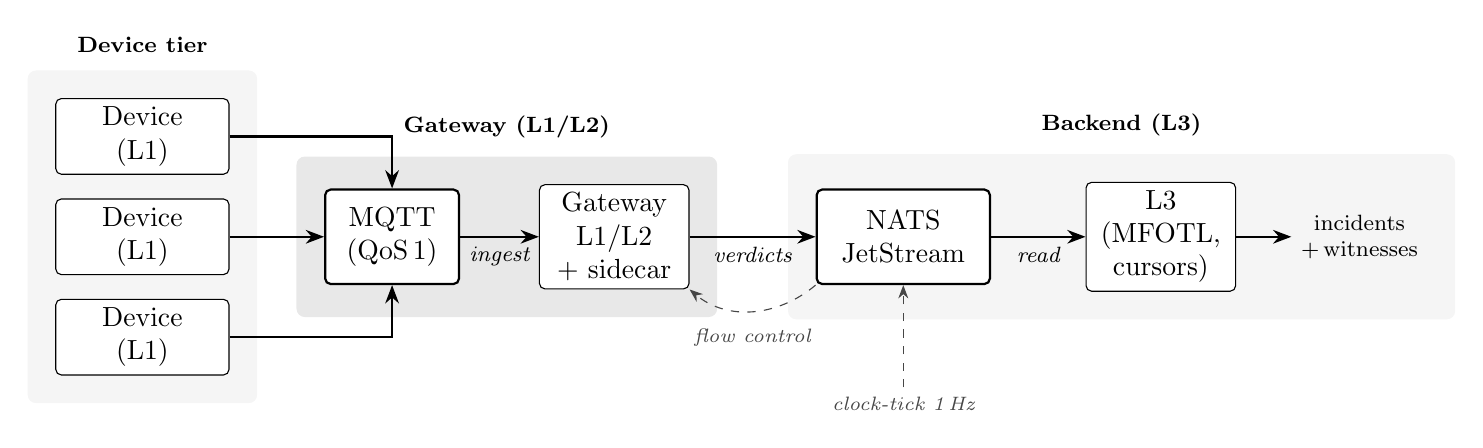
\begin{tikzpicture}[
  font=\normalsize,
  src/.style={draw, fill=white, rounded corners=2pt, align=center,
              minimum height=9mm, minimum width=22mm, inner sep=3pt},
  hub/.style={draw, fill=white, thick, rounded corners=2pt, align=center,
              minimum height=12mm, minimum width=17mm, inner sep=3pt},
  proc/.style={draw, fill=white, rounded corners=2pt, align=center,
               minimum height=12mm, minimum width=19mm, inner sep=3pt},
  arrow/.style={-Stealth, thick},
  flow/.style={font=\footnotesize\itshape, align=center},
  tier/.style={font=\footnotesize\bfseries},
  band/.style={rounded corners=3pt, inner sep=3.5mm}]
\node[src] (mc)               {Device\\(L1)};
\node[src, below=3mm of mc]   (sens) {Device\\(L1)};
\node[src, below=3mm of sens] (leg)  {Device\\(L1)};
\node[hub, right=12mm of sens] (mqtt) {MQTT\\(QoS\,1)};
\node[proc, right=10mm of mqtt] (gw) {Gateway\\L1/L2\\+ sidecar};
\node[hub, right=16mm of gw, minimum width=22mm] (nats) {NATS\\JetStream};
\node[proc, right=12mm of nats] (l3) {L3\\(MFOTL,\\cursors)};
\node[right=7mm of l3, align=center, font=\footnotesize] (out) {incidents\\+\,witnesses};
\draw[arrow] (mc.east)  -| (mqtt.north);
\draw[arrow] (sens.east) -- (mqtt.west);
\draw[arrow] (leg.east)  -| (mqtt.south);
\draw[arrow] (mqtt) -- node[flow, below] {ingest} (gw);
\draw[arrow] (gw)   -- node[flow, below] {verdicts} (nats);
\draw[arrow] (nats) -- node[flow, below] {read} (l3);
\draw[arrow] (l3)   -- (out);
\node[font=\scriptsize\itshape, gray!55!black, below=13mm of nats.south]
   (tick) {clock-tick 1\,Hz};
\draw[-Stealth, dashed, thin, gray!55!black] (tick) -- (nats.south);
\draw[-Stealth, dashed, thin, gray!55!black] (nats.south west) to[out=-140, in=-40]
   node[font=\scriptsize\itshape, gray!55!black, pos=0.5, below=1mm] {flow control} (gw.south east);
% shaded tier bands (device / gateway / backend), drawn behind the boxes
\begin{scope}[on background layer]
  \node[band, fill=black!4, fit=(mc)(sens)(leg)] (bdev) {};
  \node[band, fill=black!9, fit=(mqtt)(gw)]      (bgw)  {};
  \node[band, fill=black!4, fit=(nats)(l3)(out)] (bbe)  {};
\end{scope}
\node[tier, above=1mm of bdev.north] {Device tier};
\node[tier, above=1mm of bgw.north]  {Gateway (L1/L2)};
\node[tier, above=1mm of bbe.north]  {Backend (L3)};
\end{tikzpicture}}
\caption{\sys: the three-layer RV hierarchy decoupled over a two-broker fabric.
Devices publish to a gateway-partitioned MQTT ingest (logically one broker per
gateway; the prototype realises this as per-gateway topic prefixes on one shared
broker, equivalent for message routing but without broker-level fault isolation) at QoS\,1
(at-least-once); the gateway runs L1/L2 and
a timestamping sidecar and re-publishes verdict streams to a backend NATS
JetStream cluster, from which the L3 fleet monitors consume via independent
durable cursors. A 1\,Hz clock-tick subject drives the time-triggered silent-node
monitors, and flow control defers loss under transient overload.}
\label{fig:arch}
\end{figure}

\paragraph{MQTT for device-to-gateway ingest.}
The device-to-gateway hop is constrained and lossy, so \sys uses MQTT (Mosquitto,
QoS\,1)~\cite{mqtt,mosquitto}: ubiquitous on IoT, ack-based, and low overhead.
QoS\,1 gives at-least-once delivery with explicit PUBACKs; L1 is idempotent per
$(\text{device},\text{window})$ so duplicates are harmless.

\paragraph{NATS JetStream for gateway-to-backend delivery.}
The gateway-to-backend hop must fan a gateway's verdict stream to several
independent L3 monitors without a slow one blocking the others. \sys uses NATS
JetStream~\cite{nats}: per-consumer durable cursors let each L3 monitor read at
its own pace, and a dedicated 1\,Hz tick publisher writes to a JetStream subject
as the heartbeat that time-triggered monitors need. Verdicts are keyed by
per-device subject (\texttt{gw.$\langle$id$\rangle$.verdict}), so each device's
stream stays FIFO-ordered while a wildcard subscription (\texttt{gw.*.verdict}) fans a
whole gateway's devices into one monitor. MQTT fits the constrained device hop and a
durable per-consumer log the backend; a heavier general-purpose log such as Kafka may
impose unnecessary overhead at resource-constrained gateways.

\paragraph{Timestamping sidecar.}
A sidecar co-located with each gateway stamps each event with a trusted, monotone,
microsecond-resolution gateway-\emph{ingest} time and orders by it, restoring the ordering
invariant L3 assumes at the first trust boundary. The device-reported time is retained
only for spoof detection and diagnostics, never for ordering; original device event time
is not reconstructed.

\paragraph{Durable relay and deduplication.}
On receipt the gateway assigns each verdict a persistent event id
($\langle$gw, device, seq$\rangle$) and appends it to a local \texttt{fsync}ed write-ahead
outbox \emph{before} forwarding it to JetStream; once JetStream acknowledges the durable
publish, an \texttt{fsync}ed confirmation cursor advances, so a restart replays only the
un-acked suffix (bounding recovery cost). QoS\,1 with persistent sessions protects the
device-to-broker hop; the outbox protects the gateway-to-JetStream relay against a crash.
Backend consumers deduplicate by event id, so replays never double-count, giving
exactly-once monitoring \emph{effect} over the at-least-once transport without distributed
transactions~\cite{helland2007life}. A narrow residual window remains between delivery of
the brokered verdict to the gateway relay and completion of its local WAL \texttt{fsync},
where an in-flight verdict is still in memory; Sect.~\ref{sec:eval} validates this by
injecting a crash at each relay stage.

\paragraph{Properties the fabric carries.}
End-to-end, \sys carries a hierarchical security-property
catalogue~\cite{ares2026,csr2026}: single-node checks at L1/L2 and, at L3,
cross-device correlation (P3.1--P3.4) plus a time-triggered silent-node property
(P3.5). Briefly, P3.1 flags a multi-vector advanced persistent threat (APT) on one device, P3.2 the same
attack from $\geq3$ devices, P3.3 an escalation over time, P3.4 a persistent
overflow campaign, and P3.5 a device gone silent. Each property is sound only
because a specific transport guarantee holds (Sect.~\ref{sec:guarantees}). The
multi-gateway view also lets \sys express a property the single-gateway prototype
cannot observe: P3.6 flags an overflow campaign spanning $\geq2$ distinct
gateways,
\begin{equation}
P_{3.6}\;\equiv\;\big(\mathit{cnt}\leftarrow\mathsf{CNT}\,g;\;
\text{\small ONCE}_{[0,30]}\,\mathit{overflow}(g)\big)\;\wedge\;\mathit{cnt}\ge 2,
\label{eq:p36}
\end{equation}
i.e.\ at least two distinct gateways report an overflow within a 30\,s window.
A second fabric-enabled property, P3.7, fires when an entire gateway falls silent
while the fabric's tick keeps pulsing, distinguishing gateway-level stream loss
from the silence of an individual device:
$P_{3.7}(g)\equiv(\text{\small ONCE}\,\mathit{verdict}(g))\wedge
\neg\,\text{\small ONCE}_{[0,T_{\mathrm{gw}}]}\,\mathit{verdict}(g)$, evaluated at each tick.
P3.7 is a \emph{fabric-enabled availability} property rather than an intrinsically
cross-gateway one: it requires only a clock independent of the monitored stream (unlike
P3.6, which genuinely needs $\geq2$ gateway identities). That clock is a
\emph{backend-resident} tick publisher advancing monitoring time independently of every
gateway stream, so silence-liveness survives the loss of \emph{all} gateways at once
(verified with both killed; Q4), where the earlier per-gateway tick froze.

% ============================================================================
\section{Threat Model and Trust Assumptions}
\label{sec:threatmodel}
\sys is security-monitoring infrastructure, so its guarantees must be judged against an
explicit adversary, not benign-failure assumptions alone. This section states what \sys
defends, what it trusts, and which guarantees hold against which adversary, the threat
model the continuity mechanisms of Sect.~\ref{sec:guarantees} are designed against.

\paragraph{Asset and adversary goal.}
The asset \sys protects is the \emph{monitoring verdict stream}: every
security-relevant event durably accepted into the protected path must reach the
correlator, in the trusted gateway-ingest order, and the \emph{absence} of events must
itself be observable. The IoT payload is out of scope; \sys defends the evidence about
it, not the data. The adversary's goal is to make a
genuine attack go \emph{unflagged}, by corrupting the monitor's view
(drop/reorder/replay), \emph{blinding} it (silencing a device or gateway), or
\emph{exhausting} it (overload that sheds events), the silent-degradation modes of
Sect.~\ref{sec:intro} recast as adversarial objectives.

\paragraph{Trusted computing base.}
\sys trusts the cloud backend and L3 monitors, the two brokers under their configured
durability, and each gateway's timestamping sidecar and durable outbox, a
deliberately small TCB on the operator's side. Everything device-side of a gateway,
the devices and the network links, is untrusted; link cryptography (broker TLS and
authentication) is assumed, so the network adversary can manipulate traffic but cannot
forge a broker-authenticated identity.

\begin{table}[t]
\centering
\caption{Threat model: for each adversary capability, the \sys mitigation, the
continuity mechanism (G1--G5, Sect.~\ref{sec:guarantees}) or monitored property (P3.x)
that mitigation uses, and the residual risk. Rows marked $\dagger$ lie outside the
trust boundary (assumed, not enforced).}
\label{tab:threat}
\footnotesize
\setlength{\tabcolsep}{4pt}
\begin{tabular}{@{}R{2.6cm}R{4.0cm}R{1.0cm}R{3.0cm}@{}}
\toprule
\textbf{Adversary capability} & \textbf{\sys mitigation} & \textbf{Via (G/P)} & \textbf{Residual risk} \\
\midrule
\rowcolor{rowtint}
\multicolumn{4}{@{}l}{\emph{Network adversary (untrusted links)}}\\[1pt]
drop / delay events & at-least-once (QoS\,1 \& outbox); flow control absorbs transient backlog & G1, G5 & observable retention exhaustion, then loss \\
reorder events & monotone gateway timestamps re-anchor the timeline & G2 & cross-gateway skew bounded by offset $\epsilon$ (Sect.~\ref{sec:eval}) \\
replay events & event-id dedup (idempotent monitoring effect) & n/a & ID collision / sequence-state loss; ID forgery$^\dagger$ \\
\cmidrule{1-4}
\rowcolor{rowtint}
\multicolumn{4}{@{}l}{\emph{Device adversary}}\\[1pt]
emit malicious traffic & L1/L2 checks; fleet correlation & P3.1--4 & novel behaviour outside the specifications \\
spoof its clock & sidecar ignores device time for ordering & G2 & device time trusted only for the spoof check \\
go silent (jam / DoS) & backend tick drives silent-node under total silence & G3, P3.5 & cause (fault vs.\ attack) not identified \\
\cmidrule{1-4}
\rowcolor{rowtint}
\multicolumn{4}{@{}l}{\emph{Gateway adversary}}\\[1pt]
taken dark & gateway-silence via the backend-resident tick & P3.7 & that fleet's in-flight evidence is lost \\
compromised$^\dagger$ & \emph{out of scope}: sidecar integrity trusted & n/a & full loss of that fleet's monitoring soundness \\
\bottomrule
\end{tabular}
\end{table}

\paragraph{Adversary treatment and scope.}
Table~\ref{tab:threat} maps each capability to its mitigation. The key property is that
an adversary who \emph{silences} a link cannot thereby hide the silence: P3.5/P3.7 turn
suppression into a positive detection (though evidence may be delayed during a prolonged
partition). The residual is behaviour that is malicious yet specification-conforming, the
general limit of any specification-based monitor. A gateway \emph{taken dark} is handled
(P3.7 plus outbox replay on recovery); an \emph{actively compromised} gateway forging or
suppressing its own verdicts is out of scope (its sidecar and outbox lie in the TCB), so
\sys instead bounds the blast radius by keeping fleets disjoint (Sect.~\ref{sec:impl}).

% ============================================================================
\section{Continuity Mechanisms and Their Invariants}
\label{sec:guarantees}
This section presents the continuity mechanisms \sys establishes over the two brokers,
states each as a broker-contingent invariant tied to a specific shared-log failure, and
defines the evidence-aware verdict algebra that couples them to the monitoring output.

\sys provides five continuity mechanisms, which we label as \emph{guarantees}
\textbf{G1}~Delivery, \textbf{G2}~Order, \textbf{G3}~Tick, \textbf{G4}~Isolation, and
\textbf{G5}~Flow (the letter G stands for \emph{guarantee}).
We state each as an \emph{invariant} of the fabric, but stress what kind of claim these
are: not theorems proved from first principles, but properties the underlying
individually-established components (MQTT QoS\,1, a durable stream broker, a write-ahead
outbox, deduplication, durable cursors, a heartbeat stream) already provide \emph{by
assumption}, which we compose and make contingent on those components' durability
configuration. Their value is the explicit correspondence, RV assumption $\to$ transport
property $\to$ shared-log failure closed, not new distributed-systems results.

Two of these carry the most weight. The \emph{clock-tick} mechanism is the
subtlest: a time-triggered ``no device has reported for $T_{\mathrm{dev}}$ seconds'' property cannot
fire from a shared log, because a log with no new lines produces no events to advance
the monitor's clock; a 1\,Hz tick supplies that liveness under the total network
silence a jamming or outage event produces. \emph{Flow control} (awaited
publication and durable retention) only \emph{defers} loss under transient overload
by letting events queue: sustained overload beyond the configured retention capacity,
evaluated in Q7, makes exhaustion observable but cannot preserve G1 beyond capacity.
Delivery is therefore conditional on capacity, not unconditional.

\paragraph{Guarantees as invariants.}
Write $E_{\mathrm{brk}}$ for messages the ingest broker has durably accepted,
$E_{\mathrm{gw}}$ for those the gateway receives, $E_{\mathrm{wal}}$ for verdicts
\texttt{fsync}ed to the gateway WAL, and $\hat{E}$ for what the backend L3 monitor
observes; each verdict $v$ carries a gateway timestamp $\tau(v)$. The five guarantees
are fabric invariants:
\emph{(G1)}~at-least-once on two protected segments,
$E_{\mathrm{brk}}\subseteq E_{\mathrm{gw}}$ (persistent MQTT hop, provided the broker
has durably accepted the QoS\,1 message under a persistent session) and
$E_{\mathrm{wal}}\subseteq\hat{E}$ (gateway--backend relay), so nothing durably
accepted is lost, while drops \emph{before} durable acceptance (device crash,
device-side queue, or pre-WAL window) are outside G1;
\emph{(G2)}~monotonicity, if $v_1$ is delivered before $v_2$ then
$\tau(v_1)\le\tau(v_2)$ for same-device verdicts;
\emph{(G3)}~liveness, a 1\,Hz tick drives the backend even when $\hat{E}=\emptyset$;
\emph{(G4)}~isolation, each consumer's cursor never gates the others; and
\emph{(G5)}~flow control, awaited publishes and retention queue transient overload
rather than dropping it. G1--G2 protect and re-order the monitoring view; G3--G5
enable resilient distributed operation.

\paragraph{Evidence-aware verdicts.}
The mechanisms above bound \emph{when} the input stream is trustworthy; a monitor that
keeps emitting a bare ``no violation'' after the stream is corrupted reproduces the
silent failure we set out to remove. We therefore make evidence completeness an
explicit part of the verdict semantics. Following three-valued RV
semantics~\cite{bauer2011rvltl}, which admit an \textsf{inconclusive} verdict when the
observed trace is insufficient, a verdict is a pair $V=(s,c)$ of a
\emph{security} component and an \emph{evidence-completeness} component,
\[
\begin{aligned}
  s &\in \{\mathsf{violation},\ \mathsf{no\_violation},\ \mathsf{unknown}\},\\
  c &\in \{\mathsf{sound} \succ \mathsf{degraded} \succ \mathsf{incomplete} \succ \mathsf{unavailable}\},
\end{aligned}
\]
where $c$ is derived from continuity evidence the fabric already tracks:
$c{=}\mathsf{sound}$ when every event on the protected segments is accounted for
(G1, no gap); $\mathsf{degraded}$ past a soft retention high-water mark (G5) before
any loss; $\mathsf{incomplete}$ when a sequence gap, retention overflow, or a
monotonicity violation on the consumed stream (G2) means events are provably missing or
misordered; and $\mathsf{unavailable}$ when the tick (G3) shows the
monitor live but no evidence is arriving. Crucially, $\mathsf{unavailable}$ is an
evidence-\emph{quality} tag, not a verdict: for a property whose violation \emph{is}
the absence of events (the silent-node P3.5 and gateway-silence P3.7), the tick
reliably witnesses that absence, so it yields $(\mathsf{violation},\mathsf{sound})$;
$\mathsf{unavailable}$ applies only to properties that need positive event evidence to
decide.

The two components interact by one rule that keeps security and completeness
\emph{separate} axes rather than one ad-hoc lattice. For the monotone witness
properties formalised in Prop.~\ref{prop:soundness}, a \emph{positive} finding backed
by an intact local witness is self-evidencing (the witness \emph{is} the evidence) and
remains valid under \emph{unrelated} missing evidence, so $(\mathsf{violation},c)$
stands for any $c$; a \emph{negative} finding is only as good as its input, so a
$\mathsf{no\_violation}$ over non-\textsf{sound} evidence is downgraded,
$(\mathsf{no\_violation}, c)\mapsto(\mathsf{unknown}, c)$ for $c\prec\mathsf{sound}$,
stopping a corrupted stream from yielding an unqualified all-clear.
At L3 a property spanning gateways $g_1,\dots,g_n$ carries the meet of their evidence,
$c_{\mathrm{L3}}=\min_{\preceq}\{c_{g_1},\dots,c_{g_n}\}$, so one incomplete gateway makes
a fleet-wide all-clear $\mathsf{unknown}$. We implement all four tags over the real
JetStream (event-id continuity for gaps, a consumed-stream monotonicity check for order
violations, the retention watermark for $\mathsf{degraded}$, tick-versus-evidence for
$\mathsf{unavailable}$) and confirm each on a canonical scenario: a \emph{normal} stream
stays \textsf{sound}; a \emph{retention high-water} state ($85\%$, G5) is
\textsf{degraded}; an \emph{event-id gap} (G1) is \textsf{incomplete}, downgrading a
\textsf{no\_violation} to \textsf{unknown}; and a \emph{required stream silent} under a
live tick (G3) is \textsf{unavailable}, withholding the all-clear so only tick-backed
violations stand.

\paragraph{Soundness of the verdict algebra.}
The downgrade rule is not merely a convention: it makes the algebra \emph{sound} for a
well-defined and practically dominant class of properties. Call $\varphi$ a
\emph{monotone witness property} if its satisfaction over a window is certified by a
finite set of events and preserved under supersets, i.e.\ for traces
$\hat\sigma\subseteq\sigma$, $\hat\sigma\models\varphi\Rightarrow\sigma\models\varphi$.
The counting and multi-vector L3 properties P3.1--P3.4 and P3.6 (existential
\textsc{once}-formulas over device or gateway events) are of this class. The
absence-based P3.5/P3.7 are dual: their witness is a tick-certified silence interval,
so their soundness rests on G3 rather than on G1/G5, and we treat the monotone class
here. Let $\sigma$ be the durably-accepted event stream for the monitored identities
over the window (events that reached the protected path; device-side and pre-WAL losses
lie outside G1 and hence outside this result), and $\hat\sigma=\mathrm{dedup}(\hat E)$
the stream L3 observes after event-id deduplication.

\begin{proposition}[Conditional soundness of verdicts]
\label{prop:soundness}
Assume the order guarantee G2 (so $\hat\sigma$ is order-faithful) and, for the
cross-gateway property P3.6, a bounded cross-gateway skew $\epsilon<W$; the hypothesis
$c=\mathsf{sound}$ used below itself presupposes G1, G3, and G5 over the window. For any
monotone witness property $\varphi$ and emitted verdict $V=(s,c)$:
\emph{(i)~Positive soundness.} If $s=\mathsf{violation}$ then $\sigma\models\varphi$:
with the deduplication state intact, no loss or overload manufactures a false violation.
\emph{(ii)~Negative soundness under completeness.} If $s=\mathsf{no\_violation}$ and
$c=\mathsf{sound}$ then $\sigma\not\models\varphi$; a sound all-clear agrees with the
fault-free oracle over the accepted stream.
\emph{(iii)~No silent false all-clear.} If $\sigma\models\varphi$ but the monitor would
emit $\mathsf{no\_violation}$ (a missed violation), and the loss is observable in the
evidence stream, as an event-id discontinuity (G1/G5) or an order violation on the
consumed stream (G2), then $c\prec\mathsf{sound}$, so the algebra emits
$(\mathsf{unknown},c)$ rather than an unqualified all-clear.
\end{proposition}

\begin{proof}[sketch]
\emph{(i)}~By G1 with intact event-id deduplication (exactly-once \emph{effect}),
$\hat\sigma\subseteq\sigma$: redelivery cannot inflate a count and delivery loss only
removes events, while G2 keeps the \textsc{once}-windows aligned (and, for P3.6,
$\epsilon<W$ keeps the cross-gateway window aligned). A satisfying witness
$W\subseteq\hat\sigma$ gives $W\subseteq\sigma$, hence $\sigma\models\varphi$; no crash
or overload can manufacture a false violation.
\emph{(ii)}~$c=\mathsf{sound}$ certifies, over the window, no event-id gap on the
protected segments (G1: no delivery loss), backlog below the high-water mark (G5: no
eviction), and no order violation (G2), so $\hat\sigma$ equals $\sigma$ restricted to
the window's relevant events and
$\hat\sigma\not\models\varphi\Rightarrow\sigma\not\models\varphi$.
\emph{(iii)}~Contrapositive of (ii): a missed violation means the accepted witness was
lost or misordered in $\hat\sigma$; broken event-id continuity, or an order violation
on the consumed stream, each set $c=\mathsf{incomplete}\prec\mathsf{sound}$, triggering
$(\mathsf{no\_violation},c)\mapsto(\mathsf{unknown},c)$.
\qed
\end{proof}

The dual absence-based properties P3.5/P3.7 obtain the analogous guarantee through the
tick: it certifies the silence interval, so a genuine silence yields
$(\mathsf{violation},\mathsf{sound})$, while \emph{without} the tick (G3) the silence is
unobservable and yields a silent false all-clear, the one loss class the algebra
cannot flag.

Clause~(iii) is \emph{conditional on the loss being observable}, and that condition is
necessary rather than incidental: event-id continuity makes delivery loss observable, a
consumed-stream monotonicity check makes reordering observable, and the tick makes
silence observable, so removing an input breaks the corresponding guarantee.
A transport that carries neither (the shared log) cannot lower $c$, so every missed
violation there is a silent false all-clear. The oracle experiment (Q8,
Sect.~\ref{sec:eval}) validates all three clauses empirically.


% ============================================================================
\section{Implementation}
\label{sec:impl}
This section details how the architecture of Sect.~\ref{sec:arch} is realised: the two
brokers and the naming scheme that routes events, the timestamping sidecar, the
crash-tolerant relay (a write-ahead outbox with event-id deduplication), and the mapping
onto the edge-cloud continuum. The monitors themselves are reused unchanged.

\paragraph{Brokers and subjects.}
Each gateway ingests device telemetry over MQTT (Mosquitto~\cite{mosquitto}) at QoS\,1
on topics \texttt{dev/$\langle$gw$\rangle$/$\langle$id$\rangle$/evt}; the two-gateway
testbed shares one broker with per-gateway topic prefixes (a dedicated broker per gateway
is a drop-in alternative), so a gateway consumes only the fleet homed to it. Its L1/L2
consumer re-publishes per-window verdicts to a backend NATS JetStream~\cite{nats} stream,
routed by \emph{subject}: one subject per device, plus a fleet-wide \texttt{fleet/tick}
subject carrying the 1\,Hz liveness heartbeat.

\paragraph{Monitors.}
\sys is deliberately monitor-agnostic: it reuses the L1/L2/L3 monitors of the
hierarchical design under study~\cite{ares2026,csr2026} unmodified. L1/L2 are
lightweight; L3 is the hybrid of MonPoly~\cite{monpoly} for metric first-order
correlation and RTLola~\cite{rtlola} for the time-triggered silent-node property, the
latter driven by the fabric's 1\,Hz clock-tick subject. Because only the transport
beneath them changes, the specification logic is unchanged, its temporal interpretation
anchored to the trusted gateway-ingest timeline (Sect.~\ref{sec:arch}); an operator can
adopt \sys without rewriting existing specifications. The fabric's own contribution is
the trusted delivery infrastructure around the monitors: the relay, the timestamping
stage, the tick publisher, and the backend stream.

\paragraph{Deployment topology.}
L1 runs at the edge; each gateway node runs a co-located Mosquitto broker, an L1/L2
consumer, and a sidecar over a disjoint fleet; a cloud backend runs JetStream and the L3
monitors, so gateways fail independently. The testbed instantiates two gateway nodes of
four emulated devices each feeding one backend, and scales out by adding gateway nodes.

\paragraph{Reproducibility.}
\emph{Host.} The containerised testbed runs on a single laptop, an Apple M4 Pro
MacBook Pro (12 cores: 8 performance + 4 efficiency; 24\,GB RAM; macOS~15.3), with
Docker~28.1.1. The two-host clock-skew experiment
(Sect.~\ref{sec:eval}) instead uses two separate cloud VMs
(1\,vCPU, Ubuntu~24.04, independent kernels, NTP disabled on one) to obtain real
cross-host skew.
\emph{Software.} The stack comprises Mosquitto~2 (MQTT), NATS~2 JetStream, the
Python gateway/sidecar/relay, and an L3 image that builds MonPoly (OCaml) and
RTLola (Rust) from source; emulated devices replay the workload traces. Everything is
wired with Docker Compose and a single command brings up the fabric plus a
coordinated-attack overlay. The workload is randomised, so each run exercises the full
set of L3 properties (P3.1--P3.6) rather than a fixed script. Specifications, compose
files, and monitor wiring are provided as an anonymised review artefact, released
publicly on acceptance.

% ============================================================================
\section{Evaluation on the Controlled Testbed}
\label{sec:eval}
This section evaluates whether \sys preserves its five continuity mechanisms under
fault injection and at fleet scale, and quantifies the latency and recovery cost of
doing so.

\paragraph{Testbed and methodology.}
We deploy \sys on a multi-gateway testbed: $G$ gateways each serving a share of
$N$ emulated devices that replay a documented attack and benign
workload~\cite{ares2026,csr2026}, with the brokers first colocated and then
separated by an emulated wide-area link. All components are containerised on the laptop
host detailed under Reproducibility below (Mosquitto\,2, NATS\,2 JetStream, a MonPoly/RTLola
image, small JSON payloads). Detection figures are means over five runs; per-event latency
figures (Q2) are medians over a paced sample run per link setting, with WAN delay injected
via Linux \texttt{netem}. We ask eight questions, each naming the guarantee (G1--G5) or monitored property
(P3.x) it targets:
(Q1)~\emph{correctness}: does the fabric close the documented gaps (G1--G2);
(Q2)~\emph{overhead}: what per-event latency does it add;
(Q3)~\emph{throughput}: what message rate does it sustain (G4--G5);
(Q4)~\emph{detection}: does it flag cross-tier, cross-gateway, and silent-node attacks
(P3.1--P3.7);
(Q5)~\emph{ablation}: what failure mode does removing each mechanism reintroduce
(G1--G5);
(Q6)~\emph{crash tolerance}: does the durable outbox survive a gateway crash at each
relay stage (G1);
(Q7)~\emph{overload horizon}: how long does the fabric absorb a backend outage before
continuity is lost (G5); and
(Q8)~\emph{verdict preservation}: how many true security incidents does each
configuration miss, or silently mis-report as an all-clear, relative to a fault-free
oracle (G1--G5).

\paragraph{Where the fabric differs (Q1).}
We compare \sys against the single-host shared log (the same hierarchy \emph{without} the
broker fabric), replaying one fixed $7000$-event trace through both transports at matched
load. For steady-state ingest the two are indistinguishable: \emph{both} deliver every
event to L1 ($0$ loss over $7000$ events, at $500$ and $3000$\,msg/s, five trials each).
The $\sim$1\% ingest loss reported for the earlier prototype~\cite{ares2026} did not
reproduce here, so it is a condition-specific artefact, not where the fabric differs. It
differs on three properties the evaluated shared-log design lacks. \emph{Ordering}: on the
same $1200$-verdict stream, device-time ordering leaves $76$ out of order under the
time-spoof profile, the gateway sidecar $0$. \emph{Silence-liveness}: under total silence
the shared log yields no events so P3.5 never fires, whereas the 1\,Hz tick fires it
within one tick of the $\sim$5\,s deadline. \emph{Fault-resilience}: the delivery
guarantee's real payoff is crash recovery and bounded overload (Q6, Q7).

\paragraph{Per-event latency under a wide-area link (Q2).}
We place the fabric clients behind an emulated wide-area link (Linux \texttt{netem},
one-way delay $\delta$ per hop) and measure publish-to-consume latency on each hop
(mean/p95 in ms over a paced 400-sample run). Colocated, both hops are sub-millisecond
($0.5/1.0$ MQTT, $0.9/1.8$ JetStream). The two scale differently: the MQTT
device-to-gateway hop grows as ${\approx}3\delta$ (QoS\,1's acknowledged handshake
crosses the link several times), mean $17/32/60$\,ms at $\delta{=}5/10/20$\,ms, and
the JetStream gateway-to-backend hop as ${\approx}\delta$ ($7/13/23$\,ms). Even at a
moderate $\delta{=}20$\,ms link, p95 stays under $75$\,ms, over an order of magnitude
below the second-scale L3 detection latency. Transport overhead was not the bottleneck,
and QoS\,1's steeper WAN cost buys at-least-once delivery on the lossy edge hop.

\paragraph{Throughput and fleet scale (Q3).}
A saturation sweep (one durable consumer, rising producer count) climbs from
$\sim$10.7K to a $\sim$14K\,msg/s plateau at zero loss; past the drain rate, offered
load queues rather than drops (p95 rising to $\sim$1\,s: flow control defers loss).
Emulated fleets of $250/500/1000$ devices ($\approx$2\,msg/s each) all sustain
\emph{zero loss}; at $1000$ devices the $\approx$1930\,msg/s aggregate runs at
$\sim$60\,ms p95. This validates the message-handling path at fleet scale, not the
resource limits of $1000$ physical devices; read capacity scales further via more L3
consumers.

\paragraph{Detection (Q4).}
An eight-device, two-gateway workload (mixed overflow/APT/spam/time-spoof/clean) over
five $150$\,s runs fired all six properties P3.1--P3.6 on every run ($41.6\pm2.1$
incidents). The fabric-dependent ones fired: cross-device \textbf{P3.2} and
cross-gateway \textbf{P3.6} need the backend fleet view and per-consumer cursors
(P3.6 is unobservable single-gateway), and time-triggered \textbf{P3.5} surfaces only
because the tick drives polling under silence. Taking one gateway dark mid-run,
\textbf{P3.7} flags gateway-stream loss within the $T_{\mathrm{gw}}{=}10$\,s window, distinct from
an individual device going quiet (though not identifying the cause).

\paragraph{Clock-skew resilience of P3.6 (two independent hosts).}
We validate P3.6's skew resilience on \emph{two independent machines} (cloud VMs, separate
kernels, real network, NTP disabled on gw2 so its clock diverges genuinely). A per-gateway
clock-beacon measures the realised cross-gateway offset $\epsilon$ against a backend
reference; a zero-skew control reads $\epsilon{=}0.001$\,s. Sweeping gw2's injected offset
over $0/5/10/20/35$\,s, the measured $\epsilon$ tracks it to within network jitter
($0.001/4.75/9.71/19.64/33.76$\,s), and P3.6 (``$\geq2$ gateways within $W{=}30$\,s'')
stays sound while $\epsilon<W$ (offsets up to $20$\,s) and flips once $\epsilon$ exceeds
the window ($35$\,s), as expected for a windowed property. A real cross-region WAN and
correlated multi-gateway failure remain future work (Sect.~\ref{sec:limits}).

\paragraph{Auditable witnesses.}
Every verdict carries the evidence that produced it, so an alert is a replayable record
rather than a bare flag: a P3.6 record names the distinct gateways that discharged the
campaign, a P3.5 record the device, triggering timestamp, and $\sim$5\,s detection
latency. Duplicates are recognisable by event id and the timeline reconstructable by
timestamp, so the log is auditable.

\paragraph{Failure mode on mechanism removal (Q5).}
Each guarantee is characterised by the failure its removal reintroduces
(Table~\ref{tab:ablation}), rather than by a single scalar. Consumer isolation (G4) we
measure directly: a fast L3 consumer drains $2000$ verdicts in $0.043\pm0.001$\,s (five
runs) while a slow peer ($20$\,ms/verdict) on its own durable cursor has processed only
$3$, a $\sim$940$\times$ isolation against the $40$\,s a single shared cursor would
impose by head-of-line blocking. The other four are quantified elsewhere: ordering by the
$76/1200$ Q1 violations, delivery and flow control by the crash (Q6) and overload (Q7)
experiments, and the tick by P3.5's inability to fire from a silent log. Q8 then carries
each of these transport-level failures one level up, to the security incidents each
disabled mechanism causes to be missed or silently mis-reported against a fault-free
oracle.

\begin{table}[t]
\centering
\caption{Per-mechanism ablation: the failure each continuity mechanism's removal
reintroduces, and the measured effect (with vs.\ without the mechanism). Numbers are
from the experiments cross-referenced in the last column.}
\label{tab:ablation}
\footnotesize
\setlength{\tabcolsep}{4pt}
\begin{tabular}{@{}R{2.0cm}R{4.1cm}R{4.6cm}@{}}
\toprule
\textbf{Mechanism} & \textbf{Failure on removal} & \textbf{Measured effect (with $\to$ without)} \\
\midrule
\textbf{G1}~Delivery & crash / overload loses un-acked evidence & $1$ in-flight event lost if the crash precedes WAL \texttt{fsync}, $0$ after; without the outbox the whole un-acked suffix is at risk (Q6) \\
\textbf{G2}~Order & metric monitors see a reordered stream & $0\to76$ of $1200$ timestamp-order violations (Q1) \\
\textbf{G3}~Tick & silent-node never fires under total silence & P3.5 fires within one tick $\to$ $0$ pulses / no firing when the tick is absent (\S\ref{sec:arch}) \\
\textbf{G4}~Isolation & one slow consumer stalls all (head-of-line) & fast drain $0.043$\,s $\to$ $40$\,s shared cursor ($\sim$940$\times$) (Q5) \\
\textbf{G5}~Flow & transient overload dropped, not queued & discard-new surfaces every drop $\to$ discard-old silently loses $1000/2000$ (Q7) \\
\bottomrule
\end{tabular}
\end{table}

\paragraph{Crash recovery of the durable outbox (Q6).}
We inject a hard crash (\texttt{SIGKILL}-equivalent) into the gateway relay at each of
its three stages while it relays $50$ verdicts, then restart and read the whole stream
through backend deduplication (Table~\ref{tab:crash}). A crash \emph{after} the WAL
\texttt{fsync} loses nothing: the un-acked suffix is replayed, and any resulting
duplicate is collapsed to zero double-counted incidents (exactly-once monitoring
\emph{effect}). The only loss is a crash \emph{before} the \texttt{fsync}, dropping the
single in-flight verdict still in memory, the residual window of Sect.~\ref{sec:arch}.
Recovery is linear in the un-acked backlog: worst case (a lost cursor forcing a full
replay) takes $8.8$/$95$/$474$\,ms for $100$/$1000$/$5000$ entries
($\approx$0.095\,ms/entry).

\begin{table}[t]
\centering
\caption{Q6: gateway-relay crash injected at each stage ($50$ verdicts, crash on
\#25), measured through backend event-id deduplication. \emph{Duplicate publishes} are
verdicts re-sent on restart; \emph{duplicate incidents} are those that survive
deduplication (always $0$). Only a crash before the WAL persist loses the in-flight
verdict.}
\label{tab:crash}
\footnotesize
\begin{tabular}{@{}lccc@{}}
\toprule
\textbf{Crash stage} & \textbf{Events} & \textbf{Duplicate} & \textbf{Duplicate} \\
                     & \textbf{lost}   & \textbf{publishes} & \textbf{incidents} \\
\midrule
S1: before WAL \texttt{fsync}         & \textbf{1} & 0 & 0 \\
S2: after WAL, before publish ack     & 0 & 0 & 0 \\
S3: after publish ack, before cursor  & 0 & 1 & 0 \\
\bottomrule
\end{tabular}
\\[3pt]
{\footnotesize\emph{Stages.} S1: between the gateway's delivery of the brokered verdict
and the local WAL \texttt{fsync}, when the in-flight verdict is still only in memory.
S2: persisted to the WAL but not yet acknowledged by JetStream. S3: published and
acknowledged, but the consumer cursor not yet advanced.}
\end{table}

\paragraph{Overload buffer horizon (Q7).}
Flow control defers loss only while the backend buffer holds; we measure what happens
beyond it. Filling a bounded JetStream stream ($C{=}1000$, pushed to $2C$ with no
consumer) under the two discard policies shows the operational choice sharply: default
\emph{discard-old} silently evicts $1000$ of $2000$ verdicts with $0$ publish errors,
whereas \emph{discard-new} raises $1000$ explicit publish errors, making the same loss
\emph{observable}. Crossing the soft high-water mark marks the stream \textsf{degraded};
the first rejected or evicted publication marks it \textsf{incomplete}, consistent with
the algebra of Sect.~\ref{sec:guarantees} (retaining or retrying the rejected event is
future work, Sect.~\ref{sec:limits}). The buffer absorbs an outage of
$T_{\text{buffer}}=C/R_{\text{in}}$; at the measured $1000$-device rate
($R_{\text{in}}\!\approx\!1930$\,msg/s), buffers of $10^4$/$10^5$/$10^6$ messages hold
about $5.2$/$51.8$/$518$\,s, so a million-message buffer covers an $\approx$8.6\,min
backend outage. The durable-publish ceiling ($\approx$10.7\,K\,msg/s, single producer)
is consistent with the saturation sweep above.


\paragraph{Verdict preservation against a fault-free oracle (Q8).}
The ablation (Q5) shows that removing each mechanism reintroduces a transport-level
failure; this experiment measures the consequence one level up, on the
\emph{security verdicts} themselves. We fix a seeded workload that triggers all seven
properties P3.1--P3.7 and take the incident set the \emph{unmodified} MonPoly engine
(with tick-driven reference detectors for the liveness properties P3.5/P3.7) produces
from the fault-free stream as the ground-truth \emph{oracle} $I^\star$
($|I^\star|{=}7$). We then inject one combined fault campaign: a gateway crash, an
evidence reordering, node and gateway silence, and a retention overload, each realised
by the measured behaviour of Q6--Q7 (an in-flight loss before the WAL \texttt{fsync}, a
non-monotone rejection, an absent clock, a \emph{discard-old} silent eviction). We
replay it under the shared log, the full fabric, and the fabric with each guarantee
removed. The only variable is which alerts, and in what order, reach the unmodified
detectors, so any divergence from $I^\star$ is attributable to the transport layer.
The campaign is seeded and replayed byte-identically across all seven configurations,
with each fault bound to one incident: the pre-\texttt{fsync} crash loses \texttt{e1}'s
fifth overflow (dropping P3.4's count $5\!\to\!4$, G1); \texttt{c1}'s overflow is
transposed after its time-anomaly, breaking the P3.1 window (G2); \emph{discard-old}
evicts the oldest backlog entries, dropping the P3.2 botnet count (G5); node \texttt{f1}
and gateway \texttt{gw3} go silent at fixed offsets for P3.5/P3.7 (G3); and the
cross-gateway P3.6 campaign spans two gateways. The P3.3 escalation on \texttt{d1} is a
device-local \emph{control} that no fault touches, and is the single incident the shared
log preserves. Each incident is hit by at most one fault, so the one-miss-per-mechanism
structure is a fixed property of the seeded campaign, not a per-configuration tailoring;
the exact ids, timestamps, and bindings are pinned in the artifact
(\texttt{exp\_oracle.py}). This is a controlled causal experiment across the seven
property classes, not a statistically representative detection benchmark.
Each missed incident is then labelled by the verdict algebra of
Sect.~\ref{sec:guarantees} from the state a consumer observes: a miss it downgrades to
\textsf{incomplete} is surfaced as an honest \emph{unknown}, whereas a miss it cannot
flag is a silent \emph{false all-clear}.

Table~\ref{tab:oracle} reports the outcome. The shared log preserves only $1$ of the $7$
incidents, and every one of its six misses is a silent false all-clear: it cannot express
the gateway-scoped P3.6/P3.7, has no tick for the silent-node P3.5, and drops the crash-,
reorder-, and overload-hit incidents with no signal an operator could act on. The full
fabric reproduces the oracle exactly ($7/7$, zero false all-clears), and each
single-mechanism removal bar the timeliness guarantee G4 reintroduces one class of miss:
direct causal evidence that the mechanism, not incidental engineering, preserves the
verdict. The central result is the last column: removing G1, G2, or G5 leaves the
evidence signal intact (event ids for the G1/G5 losses, the monotonicity check for the G2
reordering), so the miss is \emph{downgraded} to a flagged \textsf{unknown} rather than
reported as a clean all-clear. The exception is G3: the tick is the very liveness clock
the completeness status is computed against, so removing it makes the two silence
incidents unflaggable and they revert to false all-clears, the one loss class the algebra
cannot surface. G4 preserves the incident \emph{set} ($7/7$) but not delivery
\emph{latency}, the timeliness guarantee quantified separately above
($\sim$940$\times$ isolation).

\begin{table}[t]
\centering
\caption{Q8: fault-injected verdict preservation against the fault-free oracle
($|I^\star|{=}7$ incidents spanning P3.1--P3.7). One combined fault campaign (crash,
reorder, silence, overload) is replayed under each configuration; incident sets are
computed by the \emph{unmodified} MonPoly engine plus tick-driven reference detectors.
A \emph{false all-clear} is a missed incident the evidence algebra cannot
flag: a silent \textsf{no\_violation}; a \emph{downgraded} miss is instead surfaced
as \textsf{incomplete}.}
\label{tab:oracle}
\footnotesize
\setlength{\tabcolsep}{5pt}
\begin{tabular}{@{}R{2.9cm}ccR{1.7cm}R{2.7cm}@{}}
\toprule
\textbf{Configuration} & \textbf{Preserved} & \textbf{Missed} & \textbf{False all-clears} & \textbf{Downgraded to unknown} \\
\midrule
\rowcolor{rowtint}
\multicolumn{5}{@{}l}{\emph{Baselines}} \\
Shared log $+$ faults & $\mathbf{1/7}$ & $6$ & $\mathbf{6}$ & $0$ \\
\sys (full)           & $\mathbf{7/7}$ & $0$ & $\mathbf{0}$ & $0$ \\
\cmidrule{1-5}
\rowcolor{rowtint}
\multicolumn{5}{@{}l}{\emph{Single-mechanism ablations ($-$G$_i$)}} \\
$-$G1 durability & $6/7$ & $1$ & $0$ & $1$ (eid gap) \\
$-$G2 order      & $6/7$ & $1$ & $0$ & $1$ (order viol.) \\
$-$G3 tick       & $5/7$ & $2$ & $2$ & $0$ \\
$-$G4 isolation  & $7/7$ & $0$ & $0$ & $0$ (timeliness) \\
$-$G5 flow       & $6/7$ & $1$ & $0$ & $1$ (eid gap) \\
\bottomrule
\end{tabular}
\end{table}

\paragraph{Independent re-execution (reproducibility).}
Re-running the public implementation on a \emph{fresh single host} with native brokers
(no containers) reproduces the qualitative claims with $95\%$ CIs: $0\%$ loss at
$250/500/1000$ devices ($1997\pm20$\,msg/s, $p95$ $121\pm6$\,ms at $1000$), ingest
saturation near $7$k\,msg/s, isolation $\sim$208$\times$, and the crash result
(Table~\ref{tab:crash}) \emph{exactly}. Absolute figures are host-dependent; the
re-execution establishes reproducibility of the \emph{behaviour}.

% ============================================================================
\section{Real-Data Validation: Water-SCADA and IoT/IIoT Datasets}
\label{sec:casestudy}
We validate the fabric on real critical-infrastructure data, replaying two
openly-published datasets, WUSTL-IIoT-2021~\cite{wustl2021} (water-supply SCADA) and
TON\_IoT~\cite{moustafa2021toniot,alsaedi2020toniot} (IoT/IIoT), through the fabric and
the real MonPoly L3 engine. \emph{Scope.} The question is transport, not detection
accuracy: whether real security-event streams can be carried and correlated end-to-end
while preserving the RV assumptions of completeness, ordering, and liveness. These are
flow logs, not distributed deployments, so they exercise detection through the unmodified
engine, not the mechanisms G1--G5 (Sect.~\ref{sec:eval}); thresholds are fixed a~priori
and untuned, and as neither dataset records a gateway assignment the cross-gateway
property runs over a \emph{synthetic} partition of source identities across two logical
gateways (Sect.~\ref{sec:limits}): each identity is hashed to one gateway independent of
label and attack class, so the partition cannot have been tuned for cross-gateway firings.

Because the device-payload predicates of Sect.~\ref{sec:eval} target application misuse
rather than network-flow malware, we add three flow monitors over \emph{failed}
connections (Zeek \texttt{conn\_state}${=}$\texttt{S0} or Argus \texttt{DstPkts}${=}0$),
applied unchanged to both datasets: \textbf{port\_scan} ($\geq20$ failed destinations in
$60$\,s), \textbf{ddos\_flood} ($\geq100$ connections to one destination in $10$\,s), and
\textbf{c2\_beacon} ($\geq50$ periodic retries, CV${<}0.5$). These feed L3 as
predicate-parametric schemas: $P3.2(A)$ fires when $\geq3$ source identities satisfy alert
$A$ in the window, $P3.6(A)$ when $\geq2$ gateways do; detection is scored per identity.

Both datasets carry and correlate end-to-end. WUSTL-IIoT-2021 is a water-SCADA Modbus
trace ($\approx$1\,M Argus flows, $6$ of $14$ source identities attacking); TON\_IoT a
UNSW cyber-range trace ($461$k records, $19$ of $11{,}536$ identities attacking over nine
classes, stressing correlation over many identities). Per-identity detection
(precision/recall, untuned) is $0.83/0.83$ (WUSTL) and $0.64/0.47$ (TON\_IoT); dedicated
detectors (e.g.\ BATADAL~\cite{taormina2018battle}) score higher. Driving the \emph{real}
MonPoly engine, the coordinated \textbf{P3.2} schema fires $2$/$11$ episodes and the
cross-gateway \textbf{P3.6} $17$/$154$ (WUSTL/TON\_IoT), at up to three coordinated sources
across two gateways, validating the fleet properties on labelled multi-source traffic.
Application-layer classes (injection, XSS, ransomware, MITM) need content-level
specifications and are out of scope. These counts are \emph{episodes} (consecutive
satisfaction timepoints collapsed), distinct coordinated events rather than
per-timepoint alerts; with the Sect.~\ref{sec:eval} monitors applied unchanged, the study
extends those controlled-testbed results to \emph{real}, labelled attack traffic
correlated end-to-end through the formal engine.

% ============================================================================
\section{Related Work}
\label{sec:related}
\sys builds directly on two recent hierarchical RV designs for edge-IoT security. The
first introduces the three-layer monitoring hierarchy and its hybrid MonPoly/RTLola
backend for fleet-wide temporal correlation~\cite{ares2026}; the second develops the
formal-methods specification of the layered security properties~\cite{csr2026}. Both
are validated as single-host prototypes reading a shared log, which leaves the delivery
layer, and thus resilience, out of scope. This paper extends that line of work by
supplying the resilient delivery layer they lack: it carries the same, unmodified
monitoring hierarchy across the edge-cloud continuum and makes the completeness of the
evidence stream part of each verdict.

The components \sys composes are individually established: MQTT QoS\,1, JetStream,
write-ahead outboxes, deduplication, durable cursors, and heartbeat streams. The
contribution is not inventing them but integrating them into a \emph{verification-aware}
fabric with an explicit correspondence among RV assumptions, transport guarantees,
adversary threats, and continuity outcomes. Against that requirement the shared-log RV
prototype~\cite{ares2026,csr2026} and MQTT-only monitoring lack durable delivery,
independent consumers, a silence-aware clock, and trusted ordering; generic stream
processors provide durability and isolation but no RV-specific ordering or
critical-infrastructure threat model; \sys supplies all five.

\paragraph{Hierarchical and spatial RV.}
STREL~\cite{strel2017} and SaSTL~\cite{sastl2020} formalise hierarchical and spatially
distributed monitoring of cyber-physical systems; the hierarchy \sys carries reuses that
decomposition pattern~\cite{ares2026,csr2026}. This line develops the \emph{logic} of
multi-tier monitoring; \sys is orthogonal, addressing how such a hierarchy is
\emph{deployed} resiliently across a real edge-cloud network.

\paragraph{Distributed, decentralised, and fault-tolerant RV.}
RV at scale has been studied at the algorithm level, in stream-based specification
languages, and in distributed and decentralised monitoring~\cite{rvsurvey,bauer2012decentralised},
and applied to CPS co-simulation and digital-twin
pipelines~\cite{temperekidis2022fmirv,temperekidis2022dt}. Closest to us is the
fault-tolerant distributed-RV line: Fraigniaud et al.\ characterise the opinions a
fault-tolerant distributed monitor needs~\cite{fraigniaud2014opinions}, Bonakdarpour et
al.\ give crash-resilient decentralised algorithms~\cite{bonakdarpour2016decentralized},
and Basin et al.\ monitor MFOTL over \emph{out-of-order} streams~\cite{basin2017outoforder}.
That work makes the monitoring \emph{logic} fault- or reordering-tolerant while
abstracting the transport; \sys sits below it, making the \emph{delivery layer's} loss,
ordering, and liveness properties first-class and measurable, so the stream those
algorithms consume is the stream their correctness assumes.

\paragraph{Cloud-native messaging and critical-infrastructure security.}
MQTT~\cite{mqtt,mosquitto}, NATS~\cite{nats}, and Kafka~\cite{kafka} are the standard
cloud-native telemetry transports; \sys repurposes this layer for \emph{verification},
requiring the five guarantees of Sect.~\ref{sec:guarantees} rather than best-effort
delivery. Orthogonally, IoT security monitoring spans surveys~\cite{cavalli2024iotsec},
ML intrusion detection~\cite{santhoshkumar2023mliot}, and attack-path analysis across
critical infrastructures~\cite{stellios2018iot} over the edge-cloud
continuum~\cite{shi2016edge}. The tiered pattern recurs across sectors (water and
IoT/IIoT here, equally rail/transport SCADA, healthcare-IoT, building automation), so
the delivery-layer guarantees are sector-independent; \sys contributes that
verification-grade delivery layer, not the detection or resource-management logic.

% ============================================================================
\section{Limitations and Threats to Validity}
\label{sec:limits}
\emph{Testbed scope.} The throughput, crash-recovery, and detection experiments run on a
single containerised host, so their absolute figures are indicative and crash tests cover
one gateway's relay path, not correlated multi-gateway failure. P3.6's skew resilience,
however, is measured across \emph{two independent machines} with separate kernels and a
real network (Q4), validated against an $\epsilon{\approx}0$ control;
the remaining threads are a real cross-region WAN (the two hosts are same-region) and
correlated multi-gateway partition. \emph{Clock-tick source.} The tick is
backend-resident, so silence-liveness survives the loss of every gateway (verified with
both killed); the residual dependency is the backend, which a production deployment should
replicate. \emph{Trusted gateway boundary.} The sidecar and outbox lie inside the trusted
computing base, so a compromised gateway that emits plausible heartbeats while
suppressing or forging evidence is out of scope: \sys detects a gateway that goes
\emph{silent} (P3.7) but not one that lies. Narrowing this, e.g.\ with hash-linked
event-sequence commitments or signed evidence receipts that make suppression
tamper-evident, is a natural next step. \emph{Real-data study.} It validates that the
fleet properties fire end-to-end on real traces, not the continuity mechanisms; the
cross-gateway result uses a synthetic gateway partition and detection is untuned. The
deterministic crash/ordering counts (Q1, Q6) reproduce exactly; stochastic figures carry
$95\%$ intervals in Sect.~\ref{sec:eval}.

% ============================================================================
\section{Conclusion}
\label{sec:conclusion}
\sys turns a single-host, shared-log RV prototype into a resilient delivery layer for
security monitoring of critical edge-IoT deployments. Pairing MQTT and a durable stream
broker with a timestamping sidecar and a crash-tolerant outbox, packaged as five
broker-contingent continuity mechanisms, it adds crash- and overload-resilient delivery
and closes the observed ordering and silence-liveness gaps at an overhead small relative
to the second-scale detection latency. Beyond resilient transport, \sys makes evidence
completeness part of runtime-verification semantics: each verdict is qualified as sound,
degraded, incomplete, or unavailable, so faults and overload can no longer silently turn
missing evidence into a false all-clear. Measured against a fault-free oracle through the
real MonPoly engine, the full fabric preserves all seven injected incidents, whereas the
shared-log baseline preserves only one and silently misreports the other six as
all-clears; and each disabled mechanism maps to one specific, measurable class of loss
(Sect.~\ref{sec:eval}). This explicit, empirically
validated link between transport continuity and verdict trustworthiness is, we argue, the
missing resilience layer between mature hierarchical RV logic and its deployment on real
critical infrastructure.

\bibliographystyle{splncs04}
\bibliography{references}

\end{document}
